

\begin{figure*}
	\centering
	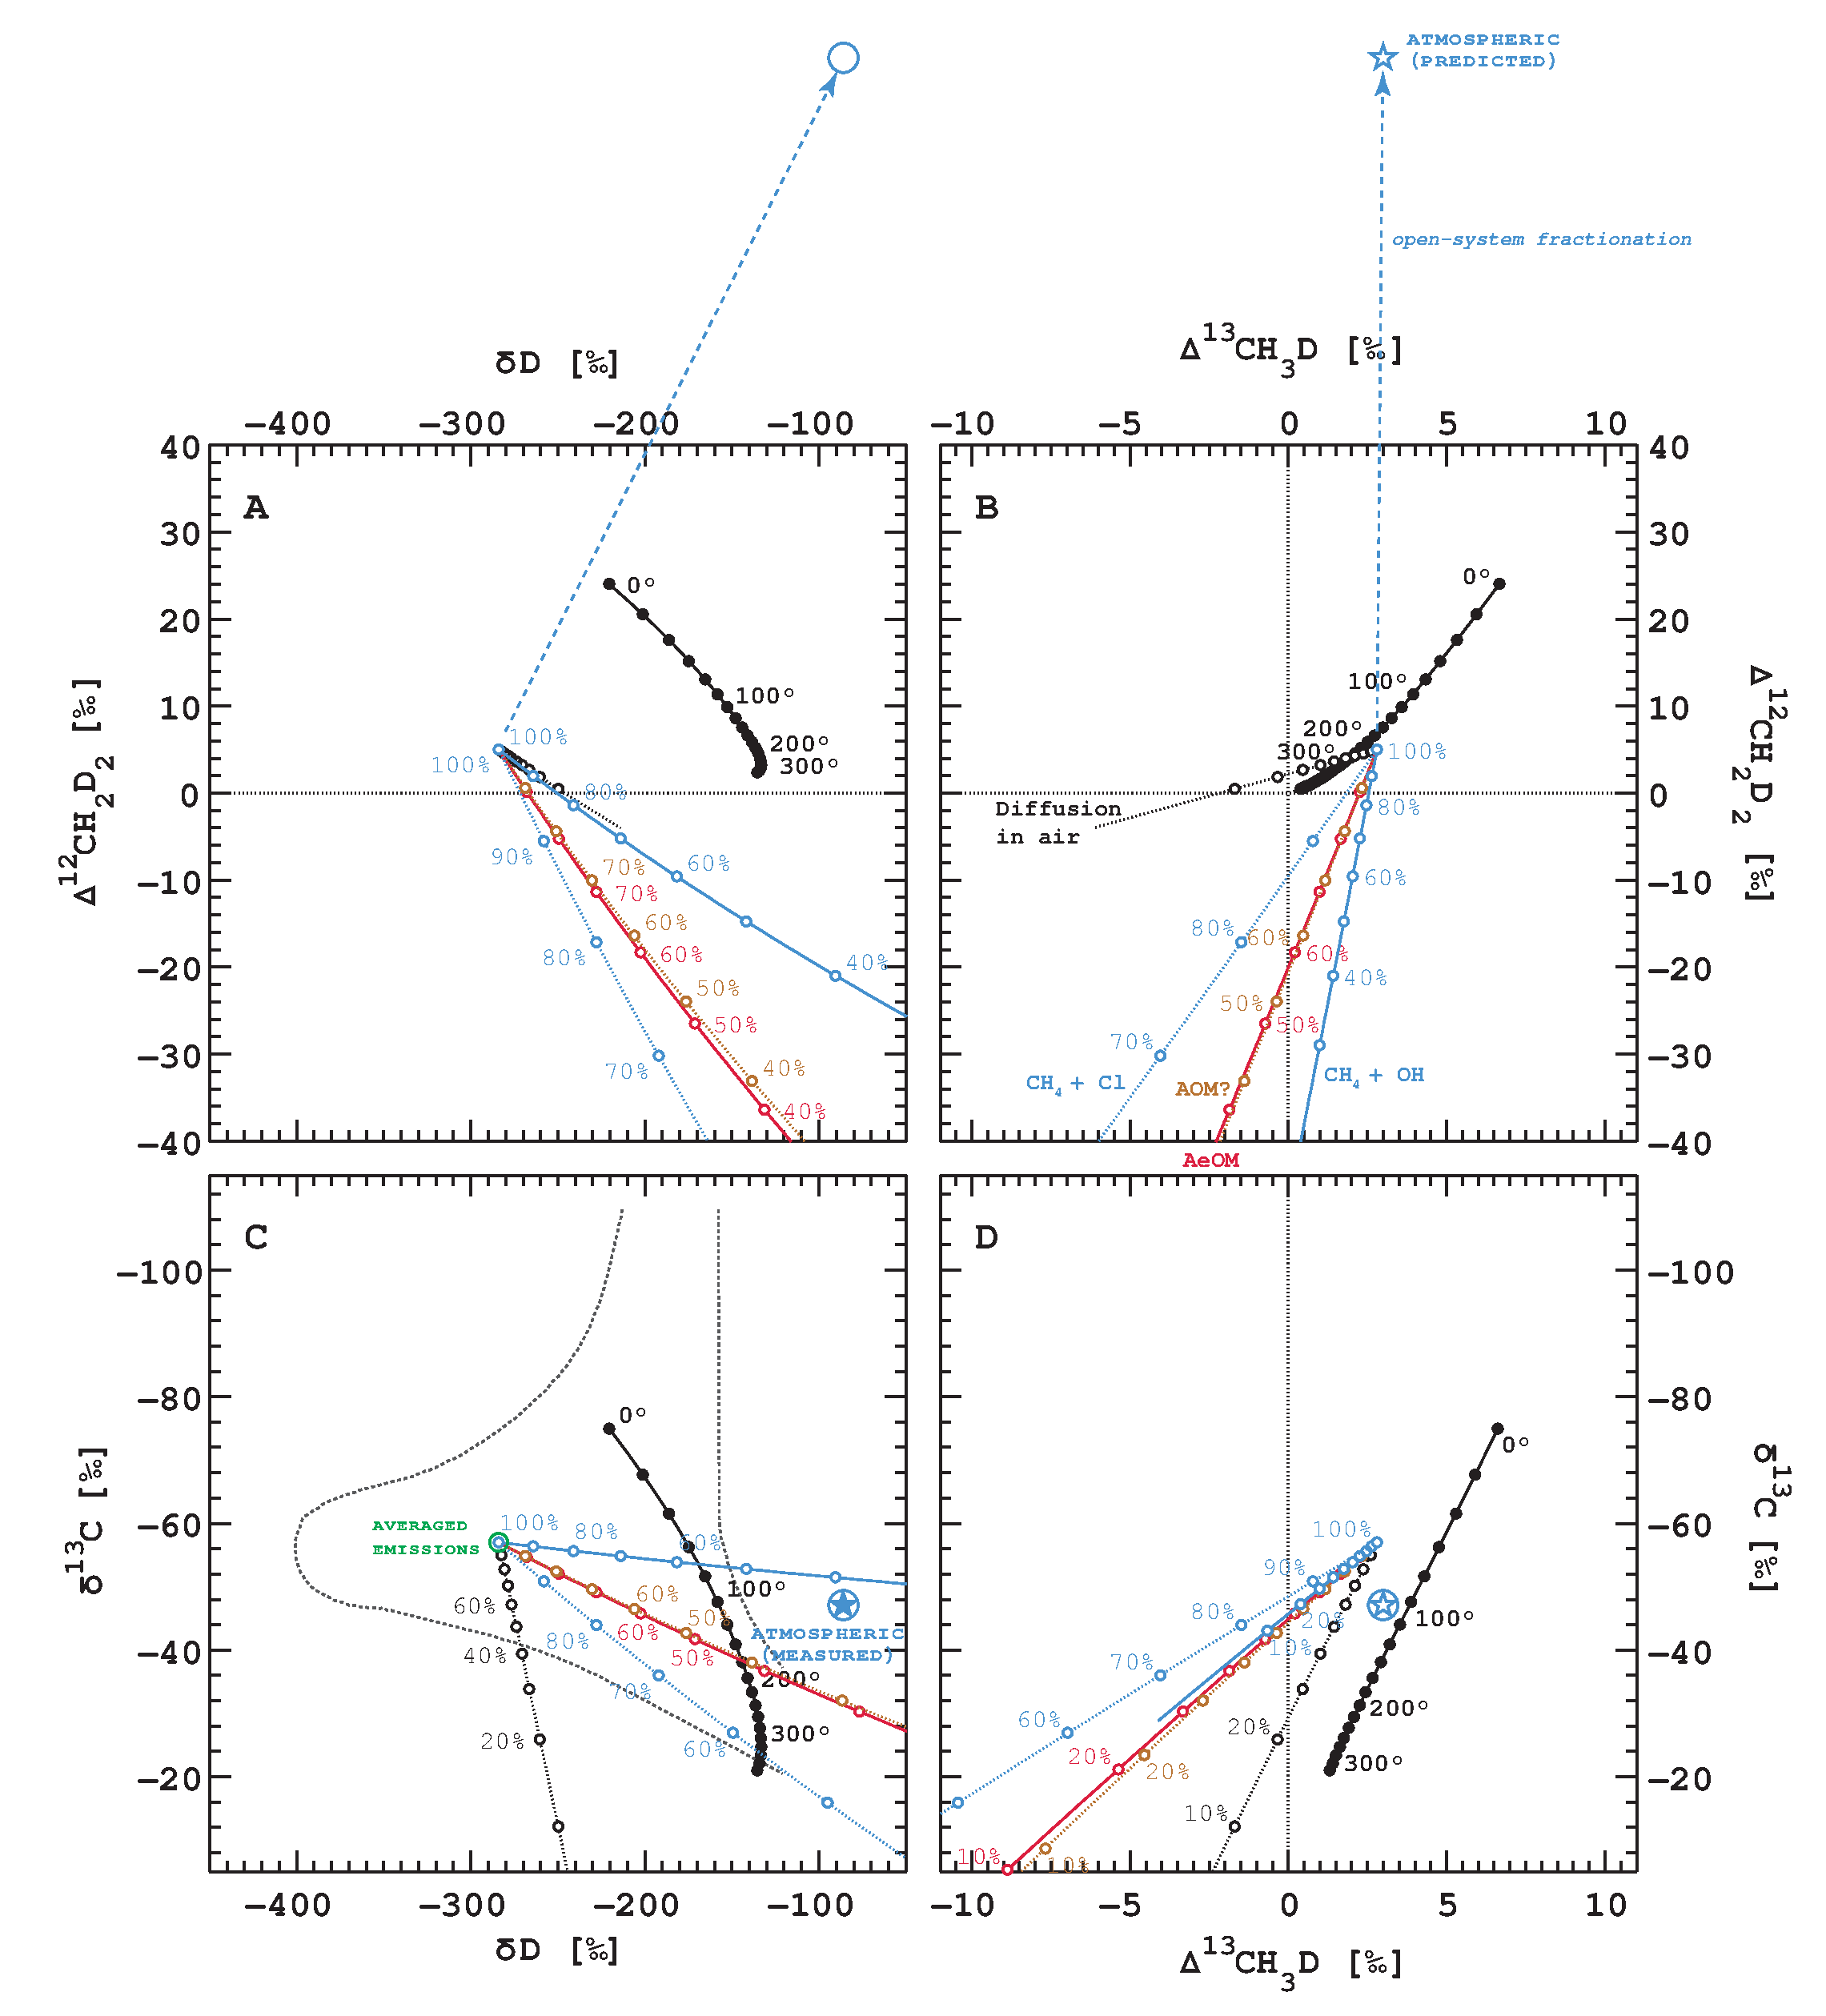
\includegraphics[scale=0.42]{figures/Fig5.5.pdf}
%	\captionsetup{format=myformat}	% hrule beneath caption
	\caption[Behavior of methane isotopologues during methane breakdown]{Evolution of CH\textsubscript{4} isotopologue ratios in
		closed-system, unidirectional bond-breaking processes. Predictions are
		derived from models and/or data presented by the MIT and UCLA teams
		\parencite{Wang++_2016_GCA,Whitehill++_2017_GCA,Young++_2017_GCA}.
		Calculations used the estimated weighted average of modern sources of
		atmospheric methane as the starting point. Trajectory labels indicate
		the fraction of remaining CH\textsubscript{4}. Predictions of
		atmospheric Δ\textsuperscript{13}CH\textsubscript{3}D and
		Δ\textsuperscript{12}CH\textsubscript{2}D\textsubscript{2} assume an
		open system in steady-state. Note that partial reversibility of the
		depicted processes will tend to pull the vectors towards the equilibrium
		line.}
	\label{fig:5:5}
\end{figure*}